% !TeX root = ../../../main.tex
\section{Results}
\label{sec:results}

Fig.~\ref{fig:tintDistrib} shows, for the eight evaluated DoPIo beam sequences using the simulated materials that were not included in the empirical model development, distributions of times-intersect measured at a depth of 25.00 mm versus shear elastic modulus. The normalized differences between those distributions (Hedge's $g$ effect sizes) and $p$-values indicating the probability of null hypotheses (Kruskal-Wallis test with Bonferroni posthoc correction) are shown in Fig.~\ref{fig:tintStat}.

\begin{figure}[htbp]
    \centering
    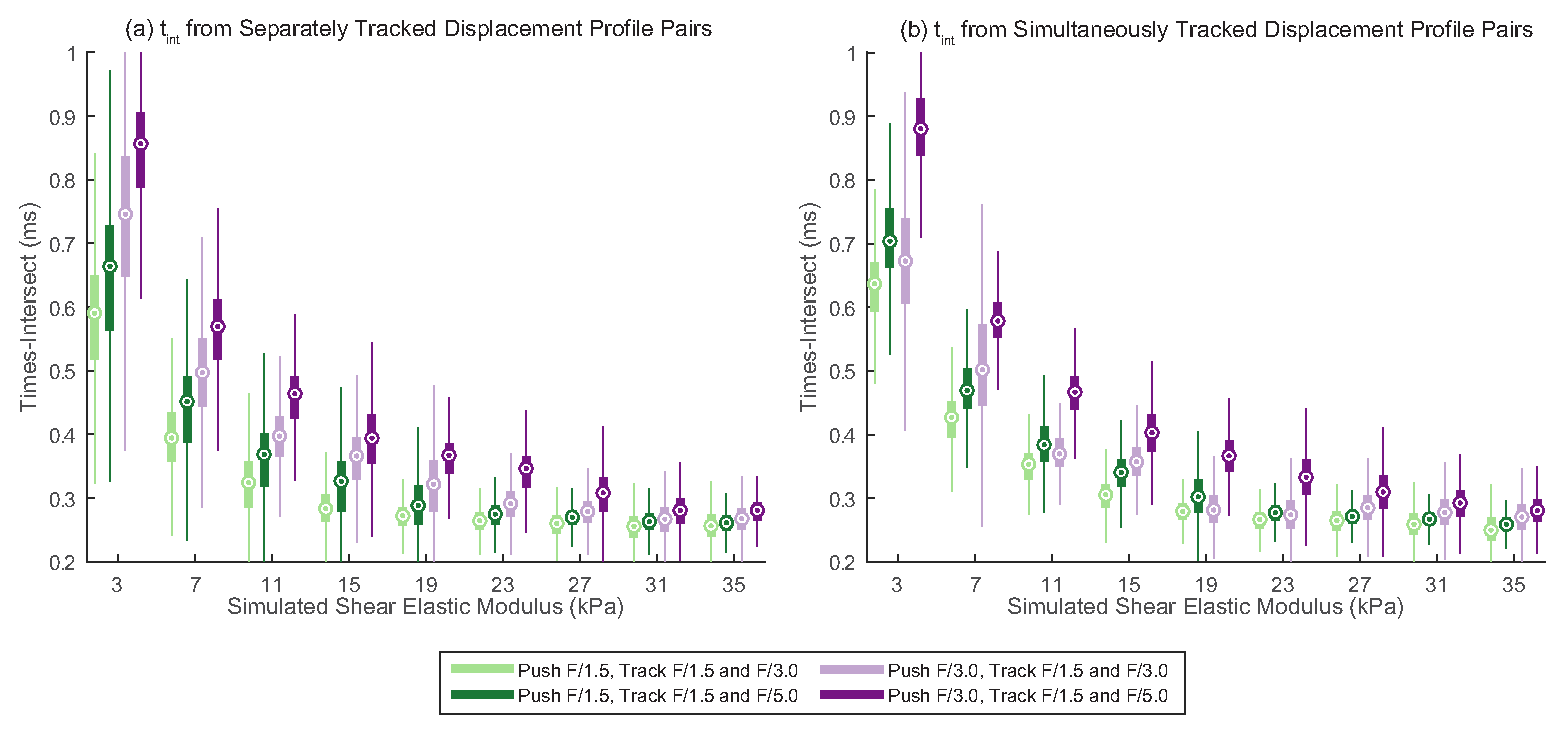
\includegraphics[width=\linewidth]{parts/dopio/fig/tint-focus.eps}
    \caption{Distributions of times-intersect values for simulated materials with varying elasticities, obtained using (a) separate or (b) simultaneous displacement tracking. Box plots show the median, interquartile range, 95\% confidence interval, and outliers for displacements measured at the focal depth (25 mm) across 20 independent scatterer realizations. Color and shading denote ARF push and tracking beam combinations as indicated in the legend.}
    \label{fig:tintDistrib}
\end{figure}

\begin{figure}[htbp]
    \centering
    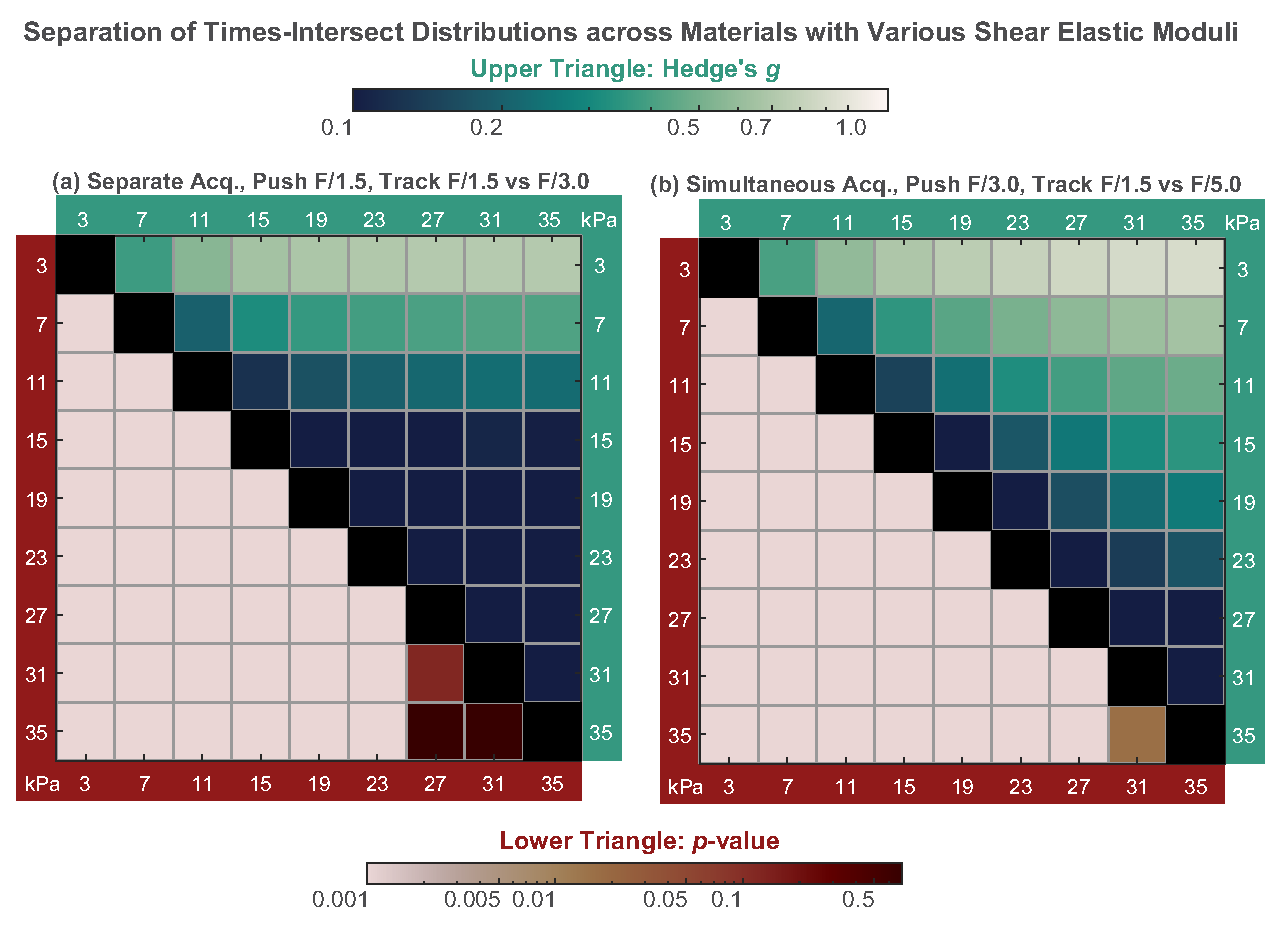
\includegraphics[width=\linewidth]{parts/dopio/fig/tint-focus-separability-modified-ltd.eps}
    \caption{Statistical comparisons of times-intersect distributions between the simulated materials in Fig. 3, with $p$-values (Kruskal-Wallis test with Bonferroni post-hoc corrections) on the lower triangle of each grid and Hedge's $g$ effect sizes on the upper triangle. Results are shown for the focal configuration pairings achieving the greatest separation between materials for (a) separate tracking (F/1.5 push and F/1.5 and F/3.0 track beams) and (b) simultaneous tracking (F/3.0 push and F/1.5 and F/5.0 track beams). }
    \label{fig:tintStat}
\end{figure}

Table~\ref{tbl:modelr2} lists the coefficients of determination ($R^2$) for the line fits created using each beam sequence and both transformations. For every sequence, the arbitrary power model yielded higher $R^2$ values, so it was selected for modulus estimation \emph{in silico}, \emph{in vitro}, and \emph{ex vivo}. Using this model, Fig.~\ref{fig:Gdistrib} shows shear modulus estimates derived from the times-intersect shown in Fig.~\ref{fig:tintDistrib}. The median and median absolute deviation of shear modulus estimate errors, as well as percent median errors, are shown in Table~\ref{tbl:medianG}. Based on the this table's results, the beam sequence consisting of an F/3.0 ARF excitation with F/1.5 and F/5.0 simultaneous tracking was selected as that which best balanced modulus estimation accuracy and precision and was implemented to demonstrate DoPIo \emph{in vitro} and \emph{ex vivo}.

\begin{table}[htbp]
    \caption{Coefficients of Determination ($R^2$) between True Elastic Modulus and $t_{\mathrm{int}}$ Transforms Assessed at the Focal Depth (25 mm) for Separate versus Simultaneous Tracking across Various Beam Sequences \emph{In Silico}}
    \centering
    \begin{tabular}{lllrr}
    $t_{\mathrm{int}}$ Transform & Push F/\# & tFc & Sep. Track & Simult. Track \\ \hline
    \multirow{4}{*}{\shortstack[l]{Inverse Sq.\\(Eq. 2)}} & \multirow{2}{*}{1.5} & 1.5 and 3.0 & 0.525 & 0.777 \\ \cline{3-5} 
     &  & 1.5 and 5.0 & 0.557  & 0.830 \\ \cline{2-5} 
     & \multirow{2}{*}{3.0} & 1.5 and 3.0 & 0.660 & 0.699 \\ \cline{3-5} 
     &  & 1.5 and 5.0 & 0.836 & 0.803 \\ \hline
    \multirow{4}{*}{\shortstack[l]{Arbitrary Power\\(Eq. 3)}} & \multirow{2}{*}{1.5} & 1.5 and 3.0 & 0.843 & 0.940 \\ \cline{3-5} 
     &  & 1.5 and 5.0 & 0.854 & 0.951 \\ \cline{2-5} 
     & \multirow{2}{*}{3.0} & 1.5 and 3.0 & 0.882 & 0.923 \\ \cline{3-5} 
     &  & 1.5 and 5.0 & 0.943 & 0.954 \\ \hline
    \end{tabular}
    \label{tbl:modelr2}
\end{table}

\begin{table}[htbp]
    \caption{Median \textpm{} Median Absolute Deviation of Errors between True and DoPIo-Derived Shear Elastic Modulus at the Focal Depth (25 mm) for Separate versus Simultaneous Tracking across Various Beam Sequences \emph{In Silico}}
    \centering
    \begin{tabular}{llcc}
    Push F/\#            & tFc        & Sep. Track                                                                  & Simult. Track                                                               \\ \hline
    \multirow{2}{*}{1.5} & 1.5 v. 3.0 & \begin{tabular}[c]{@{}l@{}}0.03 ± 3.63 kPa\\ 0.51 ± 24.19 \%\end{tabular}   & \begin{tabular}[c]{@{}l@{}}0.03 ± 2.39 kPa\\ 0.41 ± 16.51 \%\end{tabular}   \\ \cline{2-4} 
                        & 1.5 v. 5.0 & \begin{tabular}[c]{@{}l@{}}-0.13 ± 3.31 kPa\\ -2.13 ± 20.12 \%\end{tabular} & \begin{tabular}[c]{@{}l@{}}-0.06 ± 2.11 kPa\\ -0.94 ± 13.74 \%\end{tabular} \\ \hline
    \multirow{2}{*}{3.0} & 1.5 v. 3.0 & \begin{tabular}[c]{@{}l@{}}-0.13 ± 3.11 kPa\\ -2.01 ± 20.71 \%\end{tabular} & \begin{tabular}[c]{@{}l@{}}-0.05 ± 3.09 kPa\\ -1.27 ± 19.33 \%\end{tabular} \\ \cline{2-4} 
                        & 1.5 v. 5.0 & \begin{tabular}[c]{@{}l@{}}-0.06 ± 2.53 kPa\\ -1.00 ± 17.03 \%\end{tabular} & \begin{tabular}[c]{@{}l@{}}-0.02 ± 1.98 kPa\\ -0.50 ± 13.02 \%\end{tabular} \\ \hline
    \end{tabular}
    \label{tbl:medianG}
\end{table}

\begin{figure}[htbp]
    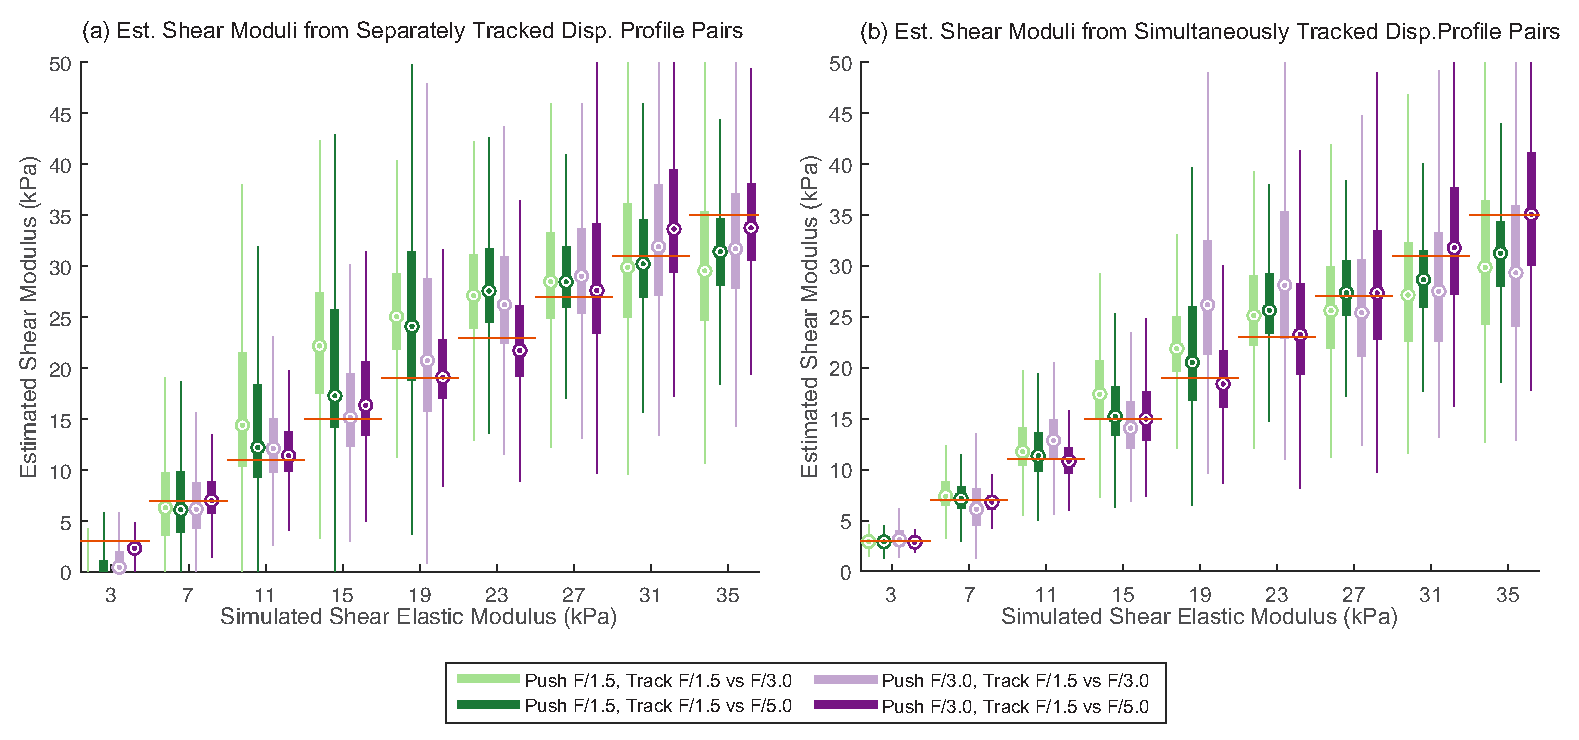
\includegraphics[width=\linewidth]{parts/dopio/fig/modulus-focus.eps}
    \caption{Distributions of DoPIo-derived elastic modulus values for simulated materials with varying elasticities, obtained using (a) separate or (b) simultaneous displacement tracking. Box plots indicate the median, interquartile range, 95\% confidence interval, and outliers for displacements measured at the focal depth (25 mm) across 20 independent scatterer realizations. Color and shading represent ARF push and tracking beam combinations, as indicated in the legend.}
    \label{fig:Gdistrib}
\end{figure}

Fig.~\ref{fig:cirsImage} depicts, for 55 V ARF excitations, DoPIo images of times-intersect and estimated shear modulus for the background and inclusions in the calibrated elasticity phantom. The estimated median and median absolute deviation of elasticity estimates were 9.0 ± 0.8 kPa in the 8.7 kPa background, 1.6 ± 0.1 kPa in the 2.2 kPa "Type 1" inclusion, 4.5 ± 0.2 kPa in the 5.1 kPa "Type 2" inclusion, and 13.0 ± 0.5 kPa in the 16.3 kPa "Type 3" inclusion, yielding contrast transfer efficiencies of 1.39, 1.19, and 1.30, respectively. The corresponding distributions of estimated moduli for all six employed ARF voltages levels, as well as example images of the Type 2 inclusion across these power levels, are shown in Fig.~\ref{fig:cirsPower} and Fig.~\ref{cirsBoxplot}. Fig.~\ref{fig:liver} depicts images of DoPIo times-intersect and estimated shear moduli in the custom liver phantom. The associated distributions of estimated moduli in the background liver tissue and the gelatin inclusion for the six ARF voltage levels are also shown, with the SWEI validation standard indicated in orange. 

\begin{figure}[htbp]
    \centering
    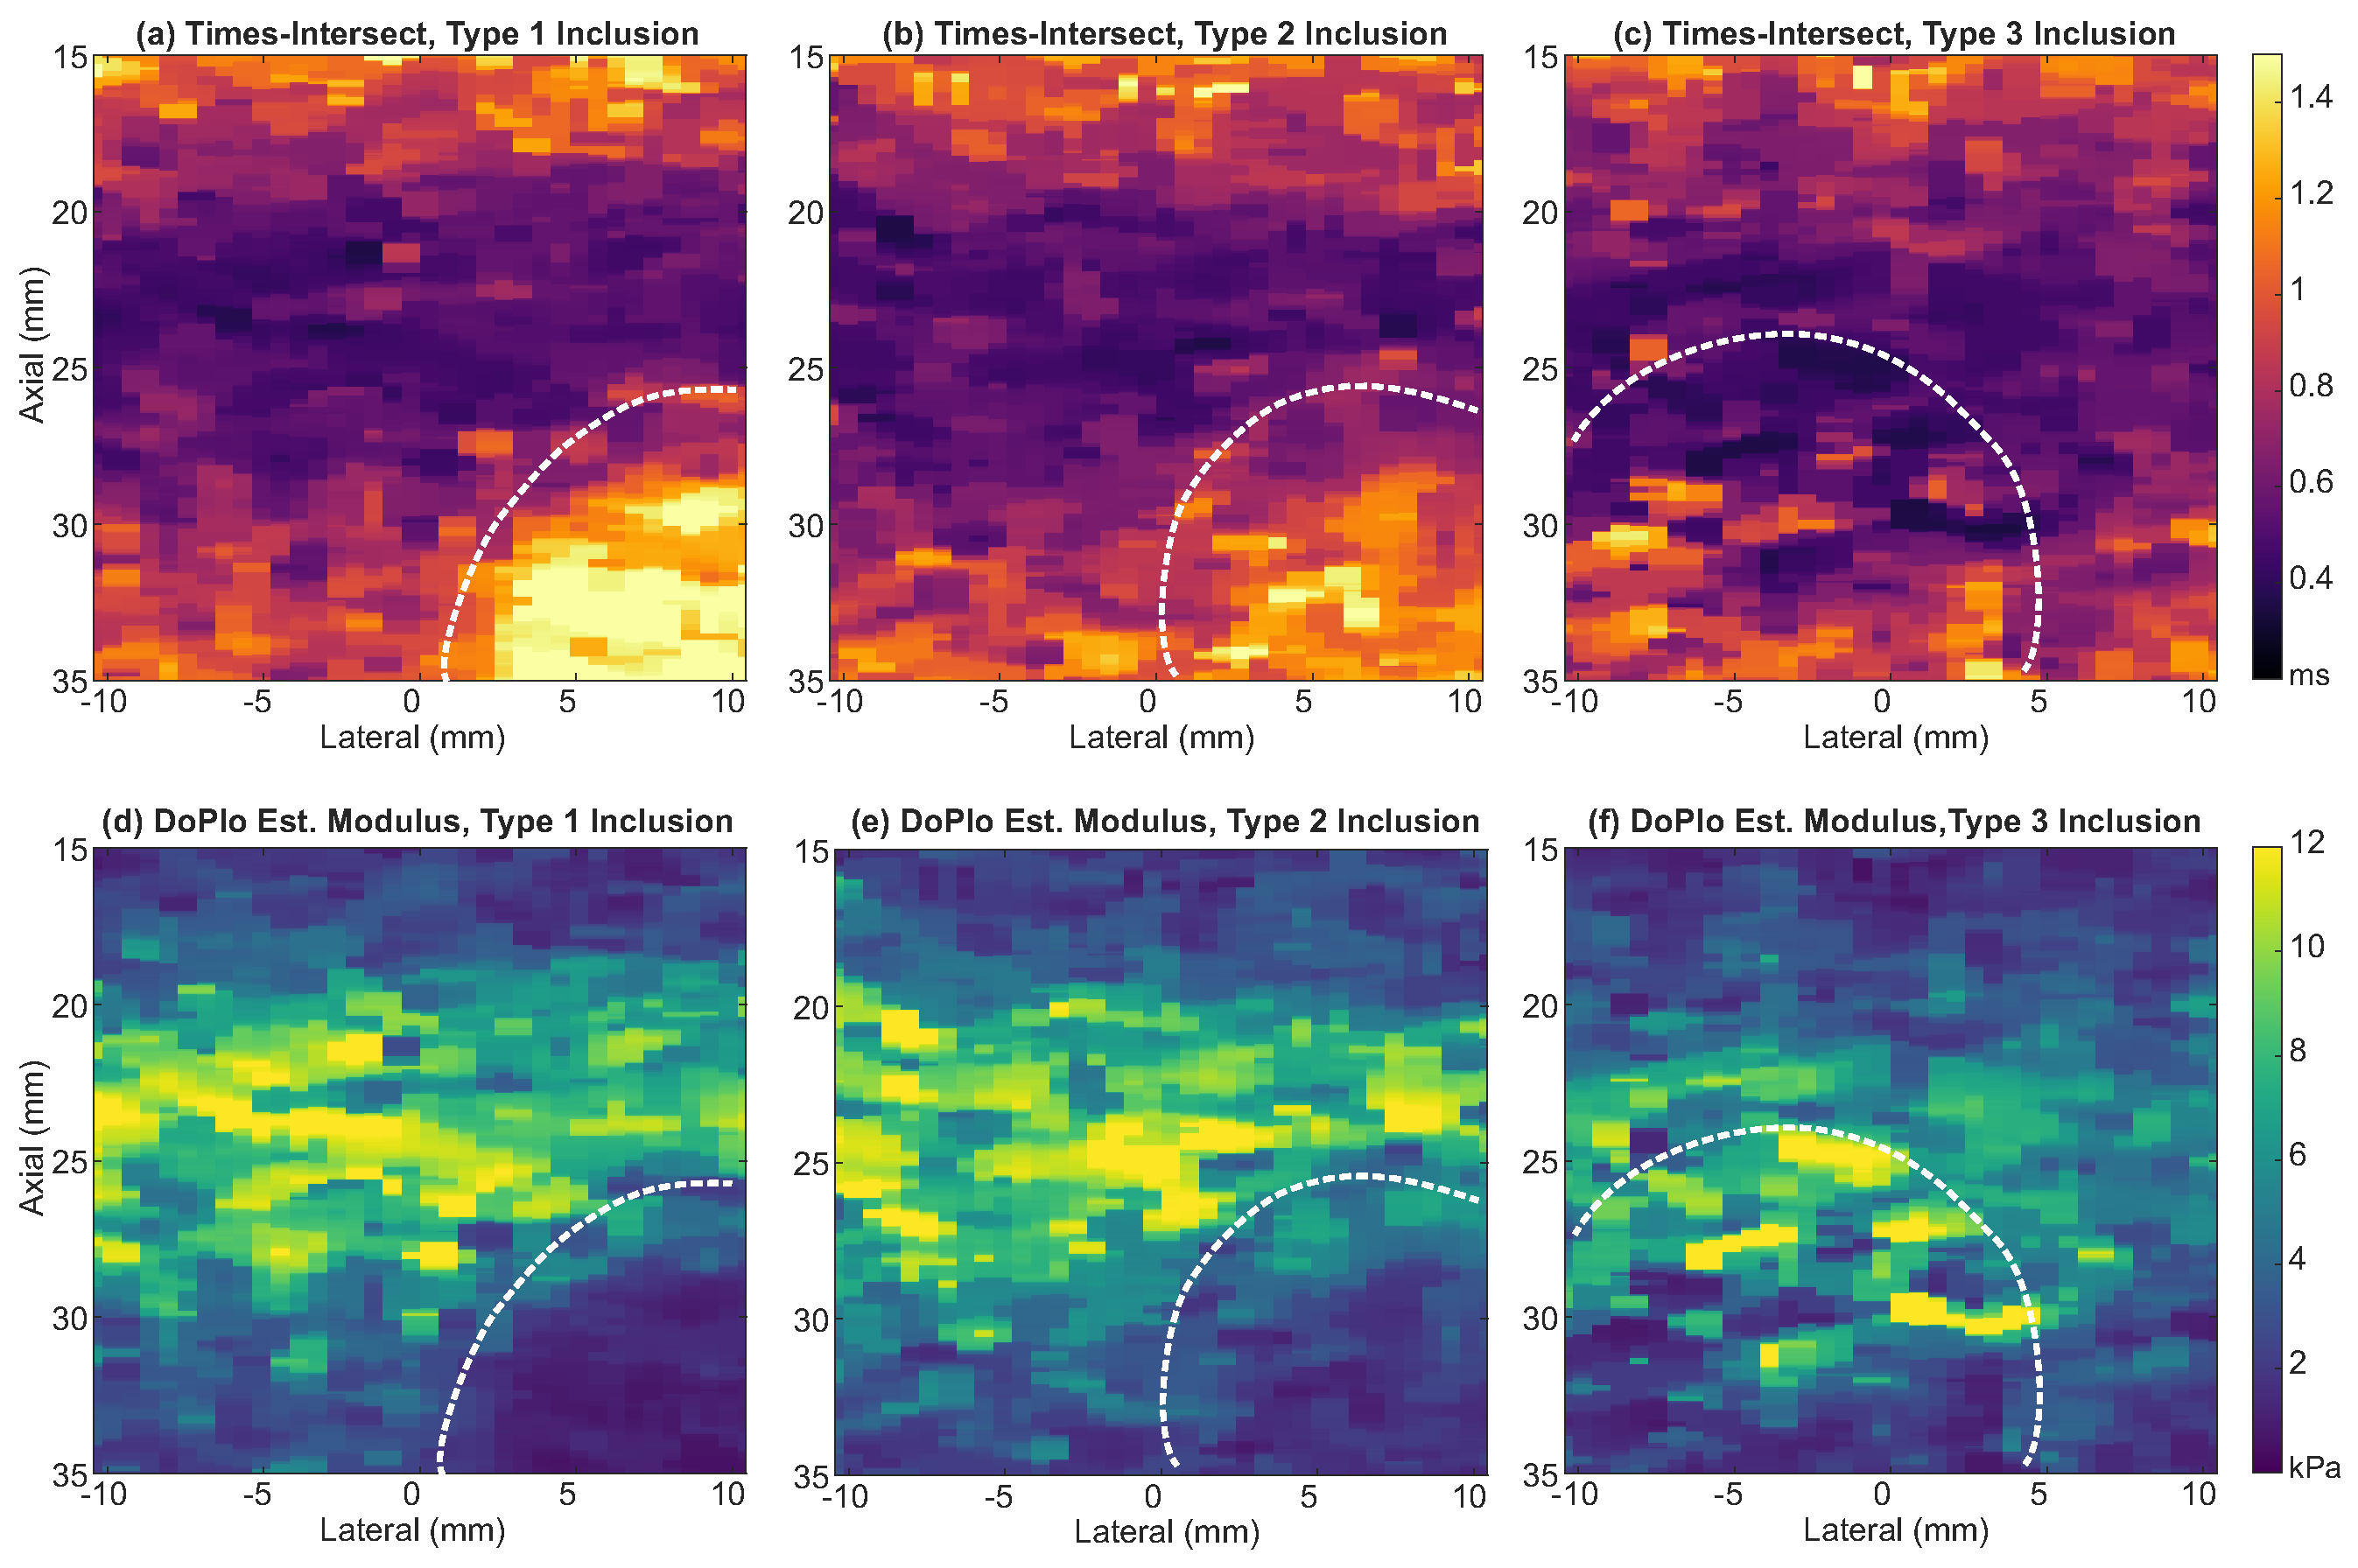
\includegraphics[width=\linewidth]{parts/dopio/fig/modulus-cirs-images.eps}
    \caption{Representative DoPIo images delineating elastic inclusions within a calibrated phantom. Panels show $t_{\mathrm{int}}$ images (a-c) and corresponding DoPIo-derived elastic modulus images (d-f) for inclusions with nominal elasticities of 2.2 kPa (a, d), 5.1 kPa (b, e), and 16.3 kPa (c, f) embedded in an 8.7 kPa background.}
    \label{fig:cirsImage}
\end{figure}

\begin{figure*}[htbp]
    \centering
    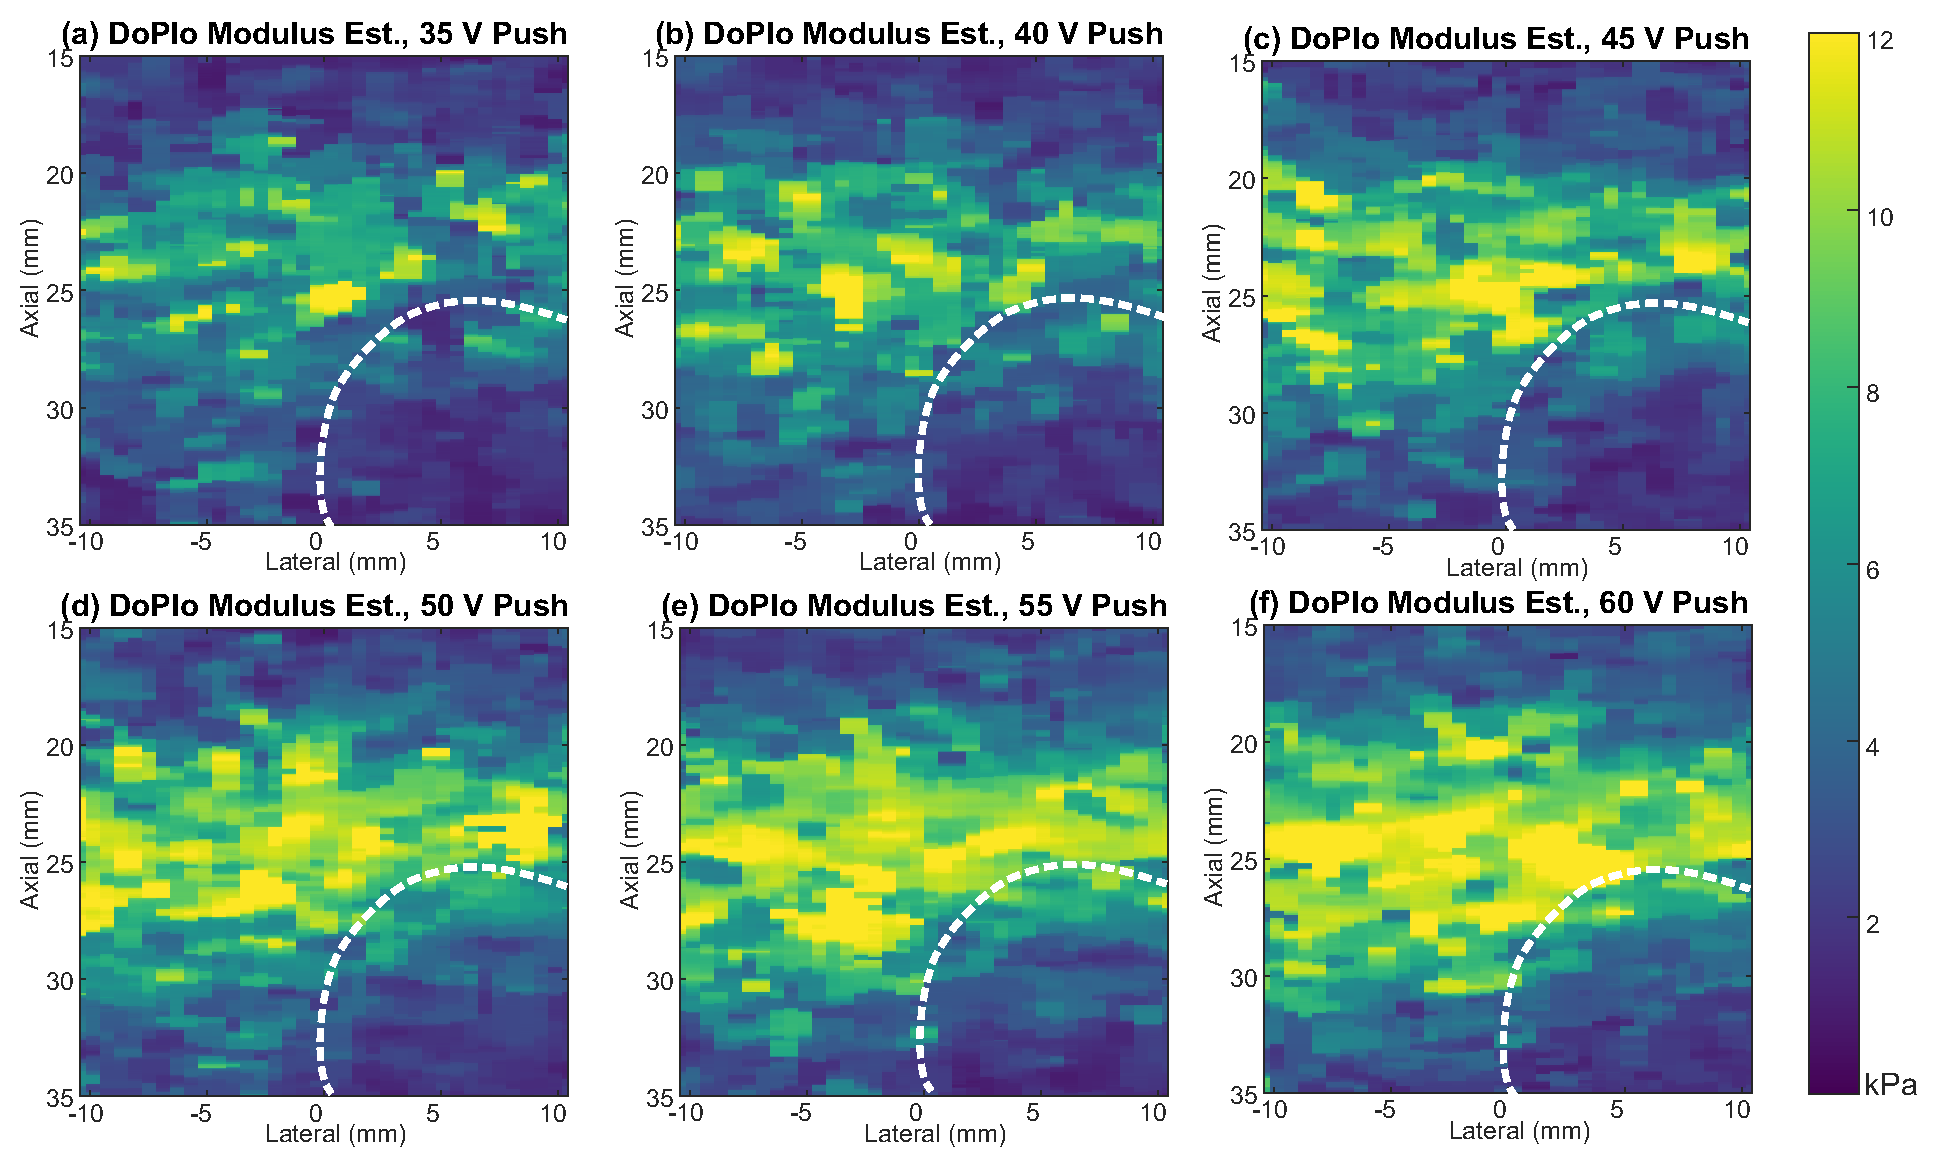
\includegraphics[width=\linewidth]{parts/dopio/fig/modulus-cirs-power.eps}
    \caption{Images of DoPIo-derived elastic modulus for a 5.1 kPa inclusion embedded in an 8.7 kPa background, obtained using ARF push amplitudes ranging from 35 V to 60 V in 5 V increments (a-f).}
    \label{fig:cirsPower}
\end{figure*}

\begin{figure*}[htbp]
    \centering
    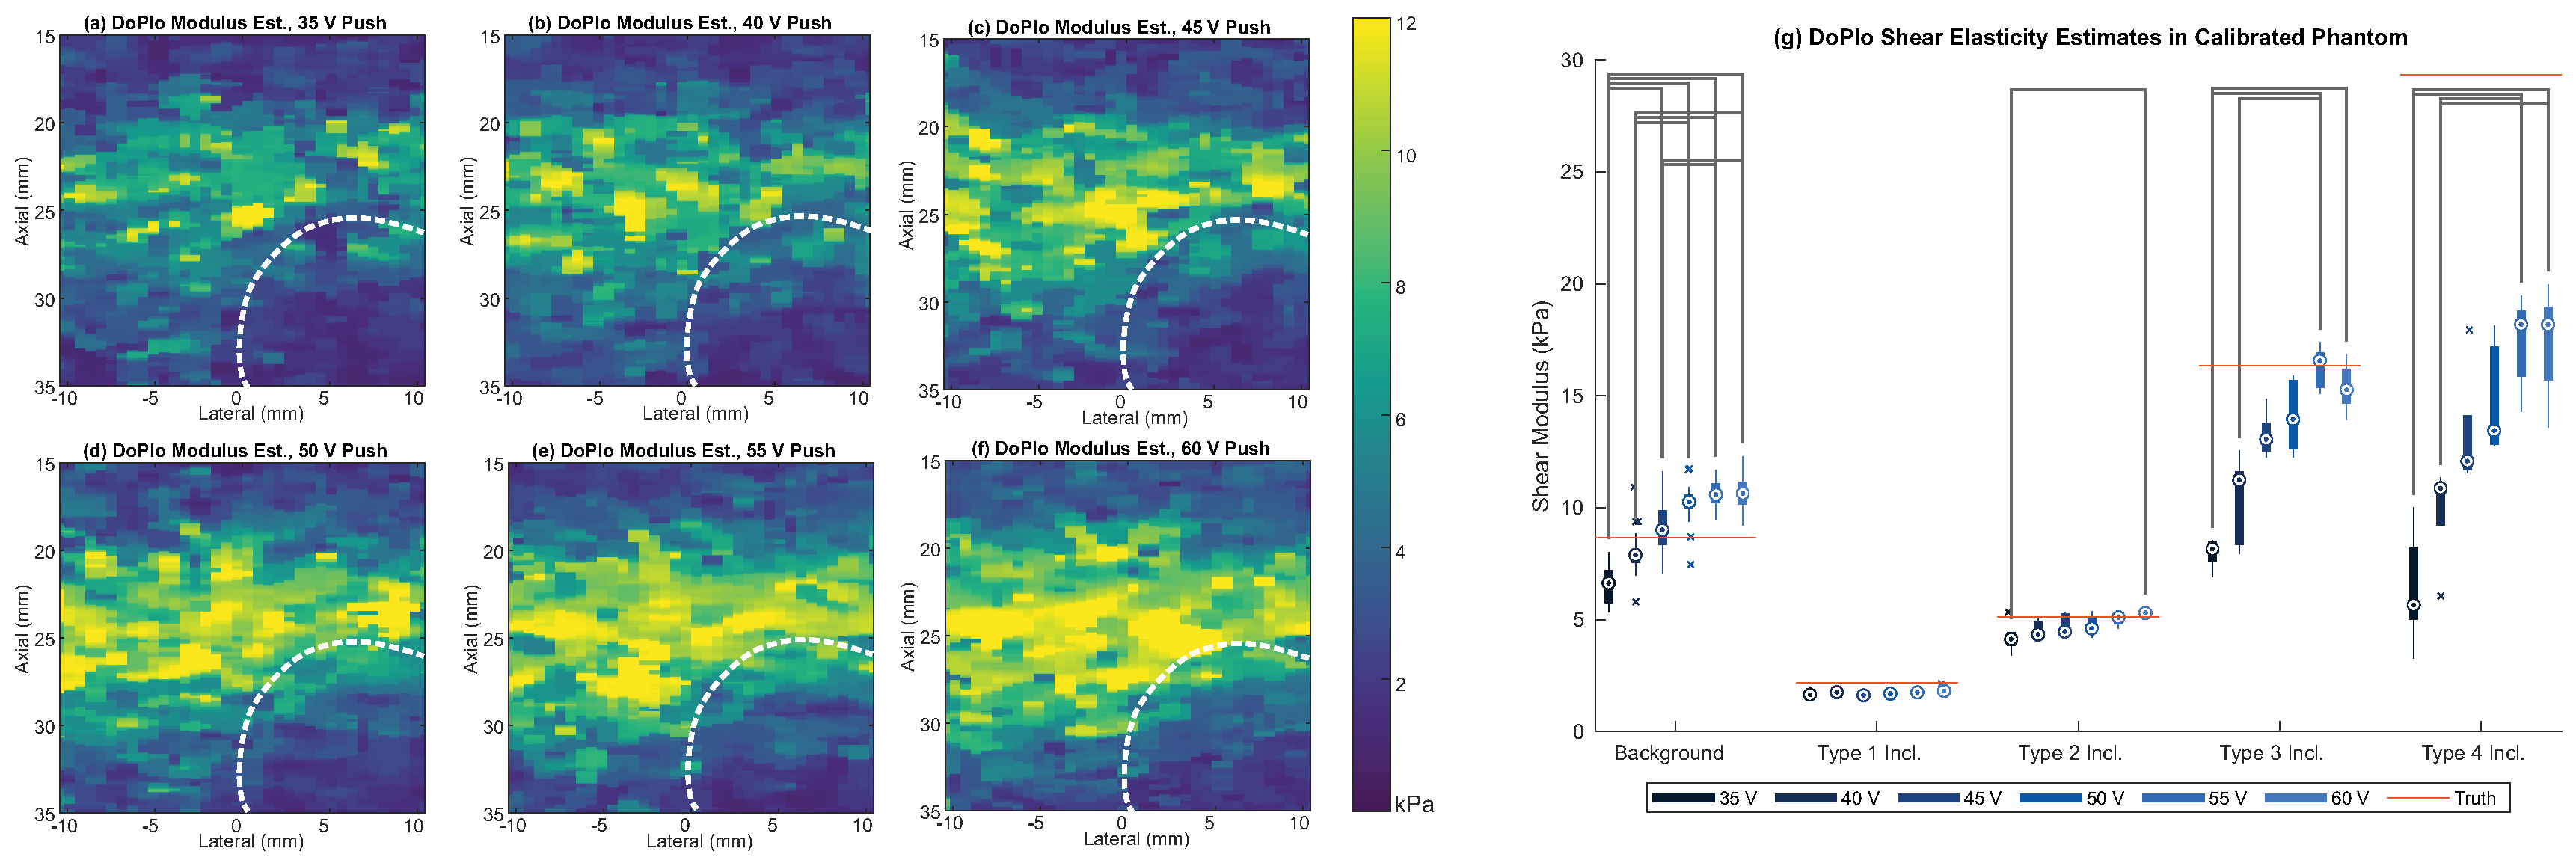
\includegraphics[width=\linewidth]{parts/dopio/fig/modulus-cirs-plot.eps}
    \caption{Box plot of DoPIo-derived elastic modulus from calibration phantom. Inclusions with nominal elasticities of 2.2 kPa, 5.1 kPa, and 16.3 kPa were imaged within the same 8.7 kPa background. Lines indicate pairs of distributions that differ significantly based on the Kruskal-Wallis test with Bonferroni post hoc correction ($p \leq 0.05$).}
    \label{fig:cirsBoxplot}
\end{figure*}

\begin{figure*}[htbp]
    \centering
    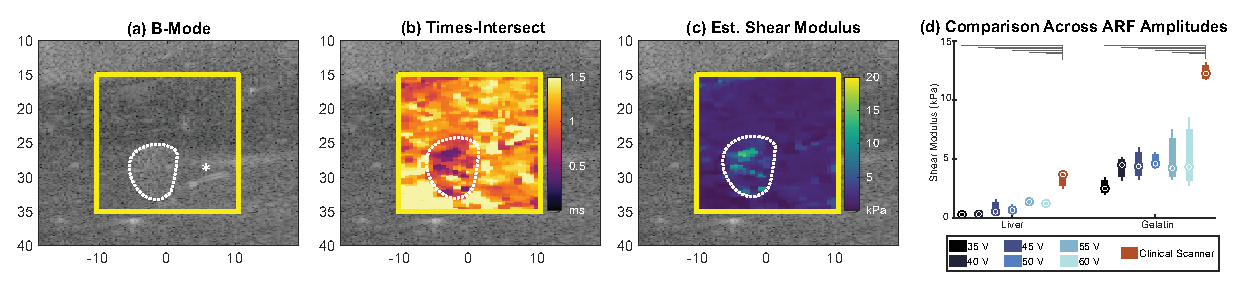
\includegraphics[width=0.8\linewidth]{parts/dopio/fig/modulus-liver.eps}
    \caption{B-mode (a), DoPIo times-intersect (b), and DoPIo-derived elastic modulus (c) images of an ex vivo porcine liver containing a gelatin inclusion. The inclusion boundary, delineated under B-mode guidance, is outlined with white dotted lines. The yellow box in (a) indicates the region used to generate the times-intersect and DoPIo modulus estimate images. Corresponding box plots of DoPIo-derived shear elastic modulus estimates (d). The orange box denotes estimates obtained using the Siemens Sequoia system, and gray lines indicate pairs of distributions that differ significantly based on the Kruskal-Wallis test with Bonferroni post hoc correction ($p \leq 0.05$).}
    \label{fig:liver}
\end{figure*}
